
\section{Experiment 2: TransFuser with one set of weights trained from scratch}
\label{sec:exp2}
For our second experiment,
we perform one full training run using the TransFuser dataset.

\subsection{Setup}
We download the original dataset\footnote{\url{https://github.com/autonomousvision/transfuser\#dataset-and-training}} and prepare a Docker container with the required dependencies.
Then, we run the provided script \texttt{team\_code\_transfuser/train.py} to train our own TransFuser.
The model is trained with the same parameters as specified in \cite{transfuser-pami}.
Using two Nvidia A100 GPUs, this took approximately 40 hours.

Using the trained model weights,
we then apply the same procedure as in \cref{sec:exp1}
to evaluate the agent's performance.


\subsection{Results}

The results from experiment 2 are shown in \cref{tab:exp2:results}.
We observe the same substitution of vehicle as in experiment 1.

\begin{table}[]
    \centering
    \begin{tabular}{|c|c|}
        \hline
        \textbf{Metric} & \textbf{Result} \\ \hline
        Routes completed & 30 / 36 \\ \hline
        Driving score & 4.27\% \\ \hline
        Route completion & 63.6\% \\ \hline
        Infraction penalty & 0.170 \\ \hline
        Collisions with pedestrians & 0.10 \\ \hline
        Collisions with vehicles & 9.2 \\ \hline
        Collisions with layout & 0.49 \\ \hline
        Red light infractions & 0.070 \\ \hline
        Stop sign infractions & 0.38 \\ \hline
        Off-road infractions & 3.0 \\ \hline
        Route deviations & 0.035 \\ \hline
        Route timeouts & 0.21 \\ \hline
        Agent blocked & 0.45 \\ \hline
    \end{tabular}
    \caption{Results from experiment 2.}
    \label{tab:exp2:results}
\end{table}

As expected, only 30 routes are completed in this experiment as well, due to the same reason as in experiment 1.

The locations of the various infractions can be seen in \cref{fig:exp2:town02}.
We see high collision densities near turns and intersections,
mostly with other vehicles.
In this case we see streaks of collisions,
where it seems like the agent continuously collides
with the vehicle in front as both drives forward. 
A video of this experiment can be found here: \url{https://youtu.be/YG6wwq1KRHM}.

\begin{figure}
    \centering
    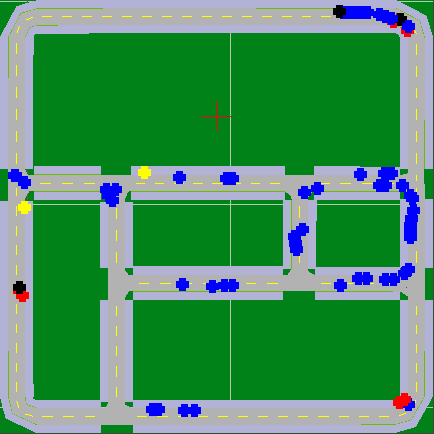
\includegraphics[width=0.5\textwidth]{chapters/4-experiments-results/figures/exp2-Town02.png}
    \caption{Infractions during experiment 2 on the Town02 map.
    Red dots are collision with the scene geometry,
    and blue with other vehicles.
    The yellow dots indicate a red light infraction,
    and the black dots mark places where the agent was permanently blocked.}
    \label{fig:exp2:town02}
\end{figure}


\subsection{Discussion}

We note overall worse results than in experiment 1.
The driving score is reduced as a consequence of lower route completion and worse infraction penalty.
Notably, the collision rate has increased,
and the agent drives more off-road.
The routes also end with the agent being blocked by an obstacle more often. 

Several reasons could be the cause of these results.
For one, deep learning will produce different sets of weights when using different random seeds,
which could result in a worse agent by pure chance.
However, in this case we are comparing an ensemble of three models to a single model,
thus the difference in performance could be due to the ensemble driving better and more consistently.

The increased collision rate also seem to be the result of continuous collision between the ego-agent and the other vehicles.
For instance, in the top right of \cref{fig:exp2:town02},
the agent is waiting in a queue and rear-ends the vehicle in front
every time the queue moves forward.
This greatly inflates the collision count,
and demonstrates a lack of proper spacing.
Similar streaks are seen elsewhere in the map.

The video shows that the agent decides independently whether to drive through an intersection,
it does not just follow the vehicle in front when it is running a red light.
This indicates that the agent has learned
a policy to stop at red lights,
instead of a policy to follow other vehicles.
However, the video also reveals an unfortunate event with a cyclist,
and the same rear-ending behaviour as seen previously.
